%!TEX root = main.tex
\begin{figure}[h!]
\centering
\vspace{-10pt}
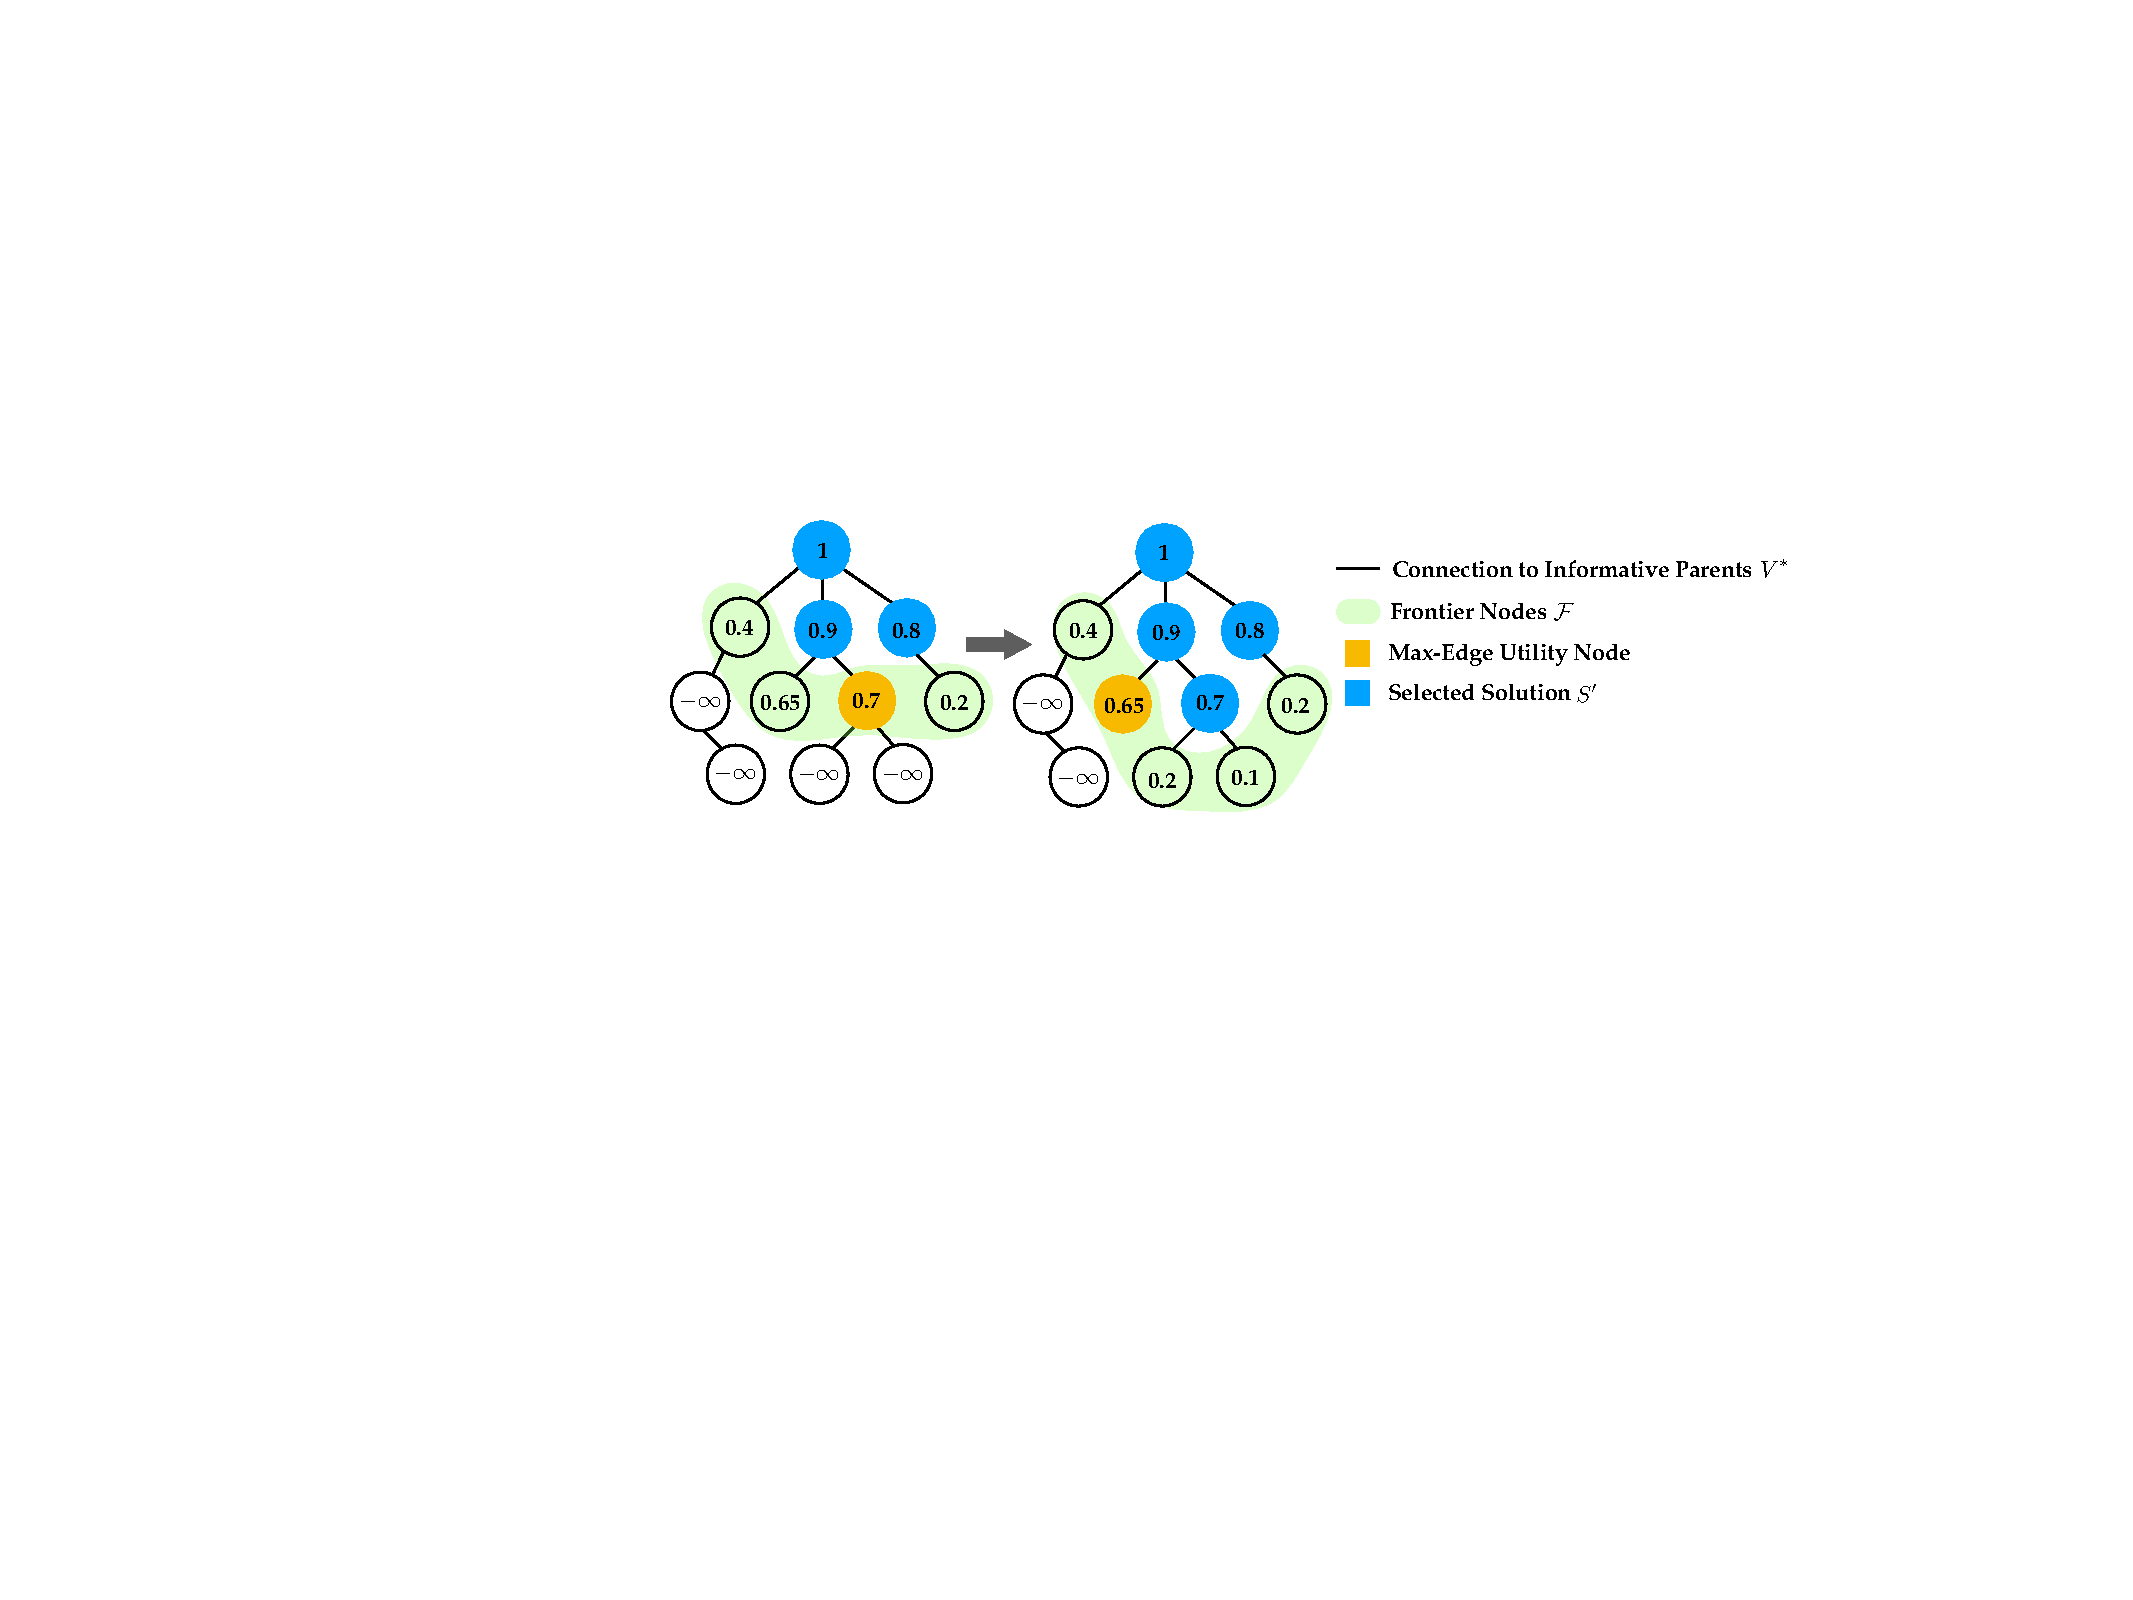
\includegraphics[width=\linewidth]{figures/frontier_greedy.pdf}
\vspace{-20pt}
\caption{Example illustrating how the frontier greedy algorithm incrementally builds up the solution by selecting the node
\change{or visualization
that leads to the highest gain in utility from the frontier at every step. Starting from a pruned lattice comprising only connections to informative parents (left) and three nodes in the existing solution (blue), we select the node with the highest utility gain (yellow) amongst the frontier nodes (green). \bchange{The contribution
to the utility of a node/visualization is depicted as the number within the node.} On the right, the newly added node results in an updated frontier and the node
leading to the highest utility gain is selected among them.
\agp{Please change "max edge utility node" to "max utility node". Can you also
add an edge between 0.8 and 0.7 so that it doesn't look like a tree? Also another edge between 0.65 to one of the -$\infty$s}}
}\dor{Changed.}
\vspace{-10pt}
\label{fig:frontier_greedy}
\end{figure}
\section{\system: Our Solution\label{sec:system}}
We present our system, \system, by first providing a high-level overview of the underlying algorithm,
and then describing the user interaction mechanisms.
\change{
  \subsection{Lattice Traversal Algorithm\label{sec:algorithms}}
  For a given dataset and user-selected X and Y axes,
  we first enumerate all possible attribute-value combinations
  (i.e., filters) to construct the lattice upfront.
  \bchange{Like we described in the previous section, we retain
  only the edges that correspond to informative parents.}
  Then, we traverse this pruned
  lattice to select the connected subgraph $S$ of $k$
  visualizations (or equivalently, nodes in the lattice)
  that maximizes
  the utility $U$.
}%generating the visualization lattice, and then present an overview of how we
\tr{
\stitle{Lattice Generation:} Our system supports two variants of traversal based on the lattice generation procedure---offline variants that first generate the complete lattice and then work towards identifying the solution with maximum combined-edge utility, and online variants that incrementally generate the lattice and simultaneously identify the solution. The offline variants are appropriate for datasets with a small number of low-cardinality attributes, where we can generate the entire lattice in a reasonable time; whereas the online variants are appropriate for datasets with many high-cardinality attributes, where we need to incrementally generate a partial lattice. \tr{
  To prevent the danger of visualizations with small population size, users can also select an \textit{iceberg condition} ($\delta$) to adjust the extent of pruning on visualizations whose sizes fall below a certain percentage of the overall population size. \footnote{The terminology is used in the discussion of iceberg cubes in OLAP literature~\cite{Xin2007}.}
}
%In most cases, the lattice contains a large number of visualizations due to the presence of many attributes or high-cardinality attributes in the dataset. In such cases finding an optimal solution is computationally challenging.
\stitle{Lattice Traversal:} We first describe the offline version of the algorithm before outlining the modification required for the online variant of the algorithm. Given a lattice that has been materialized offline,
}
\change{Our algorithm for traversing the lattice,
titled {\em frontier-greedy}, is inspired
by the notion of ``externals'' in
Parameswaran et al.~\cite{Parameswaran2010}.
The algorithm incrementally grows a subgraph $S'$ until
$k$ nodes are selected.
Throughout, the algorithm maintains a set
of {\em frontier} nodes $\mathcal{F}$---nodes
that are connected to the existing subgraph solution $S'$
but have not yet been
added. The frontier nodes includes all of the children of the nodes
in $S'$.
Given that our pruned
lattice only retains edges between children and their
informative parents, all frontier nodes are guaranteed
to have an informative parent in the the existing solution
and can be added to $S$ without violating informativeness.
%Any frontier node whose informative parent is present in the existing solution can potentially be added to the existing solution, without violating the informativeness principle.
At each iteration, the algorithm adds the node from the frontier
nodes that leads to the greatest increase in the utility of $S'$: i.e.,
the node $V_n$ such that $U(S' \cup \{V_n\})$ is the largest.
Figure~\ref{fig:frontier_greedy} displays how the algorithm
maintains the list of frontier nodes (in green), and the current $S'$ (in blue),
adding the node that leads to the greatest increase in utility (in yellow).
Algorithm~\ref{algo:frontier_greedy} provides the pseudocode.
}
\begin{algorithm}
  \begin{algorithmic}[1]
  \Procedure{PickVisualizations}{$k$, $\mathcal{L}$}
  \State $S' \gets$ \{$V_0$\}  \text{/* adding the overall node */}
  \While{$|S'| < k$}
      \State $\mathcal{F}$ $\gets$ getFrontier($S'$, $\mathcal{L}$)
      \State bestUtility $\gets$ $-\infty$
      \For{$V_i$ $\in$ $\mathcal{F}$}
      \If{$U(S' \cup \{V_i\})>$bestUtility}
      \State maxNode $\gets$ $V_i$
      \State bestUtility $\gets U(S' \cup \{V_i\})$
      \EndIf
      \EndFor
      \State $S' \gets S' \cup$ \{maxNode\}
  \EndWhile
  \Return $S'$
  \EndProcedure
  \end{algorithmic}
  \caption{Frontier Greedy Algorithm}\label{algo:frontier_greedy}
\end{algorithm}
%The frontier greedy algorithm first compiles a list of candidate nodes known as the \textit{frontier} nodes, which encompasses all nodes that are connected to the existing subgraph solution. As long as the informative parents of frontier nodes are already present in the solution, the frontier nodes can be appended to the current solution without violating requirement (ii) in the problem formulation, enforcing the presence of informative parent for every selected visualization. To obtain the frontier nodes, the algorithm scans and adds all children of leaf nodes of the current dashboard as part of the frontier. \tr{In the online version, it additionally checks for each child whether its informative parent is present in the current dashboard.} As illustrated in Figure~\ref{fig:frontier_greedy}, at each step, our algorithm greedily picks the node with the maximum edge utility amongst the eligible frontier nodes to add to the current solution, and updates the frontier accordingly. \ccut{The \textit{frontier greedy} algorithm discussed here is used for generating the dashboards for our user study and we defer the details of other algorithms that we have developed for lattice traversal to the technical report. }
%\par The frontier greedy algorithm obtains a list of candidate nodes known as the \textit{frontier} nodes, which encompasses all neighbors of nodes in the existing subgraph solution. Any of the nodes in the frontier can be added to the current solution since their informative parent is present in the solution. To obtain the frontier nodes, the algorithm scans and adds all children of leaf nodes of the current dashboard as part of the frontier. In the online version, it additionally checks for each child whether its informative parent is present in the current dashboard. At each step, our algorithm greedily picks the node with the maximum utility amongst the frontier nodes to add to the current solution, and updates the frontier accordingly. \tr{The path merging algorithm first generate the informative paths from root to every candidate node. Then, it greedily merges the paths with high-utility to create a subgraph whose size is less than or equal to maximum capacity $k$.}

\subsection{User Interaction\label{sec:interaction}}
\begin{figure*}[ht!]
\centering
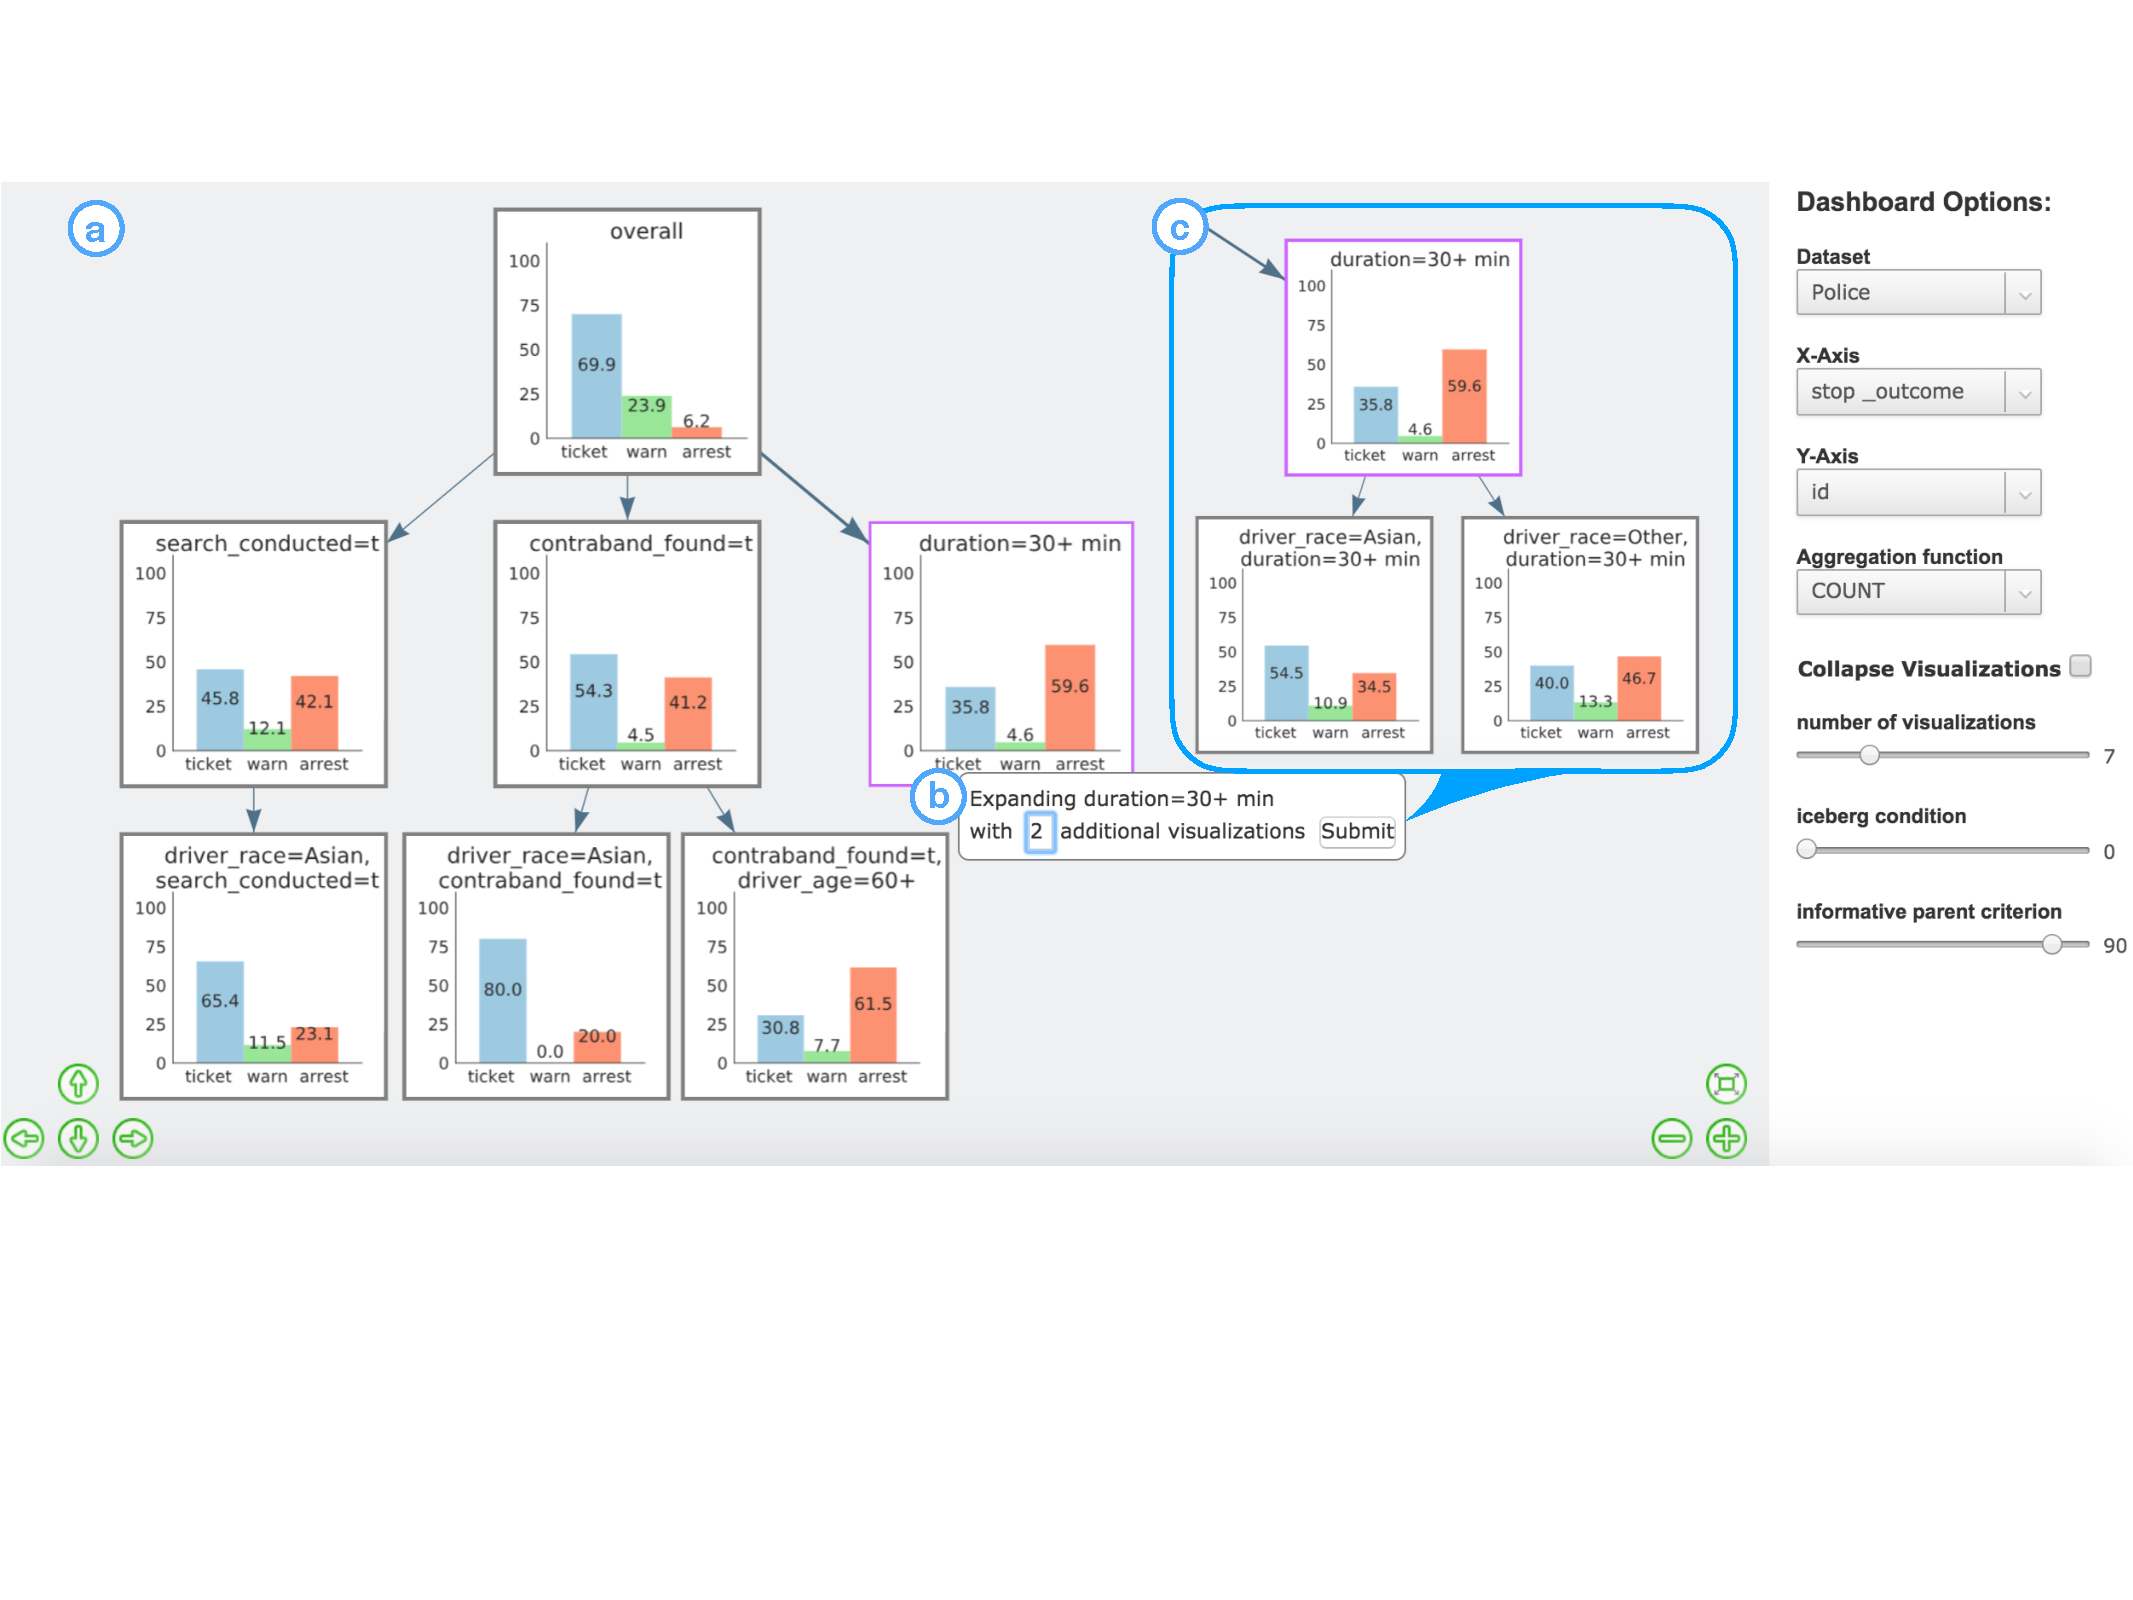
\includegraphics[width=0.9\linewidth,frame]{figures/overview_interface_expand.pdf}
\caption{a) Overview of the \system interface for the Police Stop dataset. Users can  select \change{x, y axes, and aggregation function via the dropdown menu, to define the visualization space of interest, as well as adjusting dashboard parameters, such as the number of visualizations to show in the dashboard (k) via the sliders.} b) User clicks on the duration=30+min visualization to request 2 additional visualizations. c) A preview of the added portion of the resulting dashboard is shown.}
% Default values are set for system related parameters such as the number of visualizations to show in the dashboard (k), iceberg condition for pruning ($\delta$), and informative parent criterion ($\theta$), which can be adjusted by the users via the sliders if needed.
\label{fig:overview}
\vspace{-10pt}
\end{figure*}%optional system parameter settings

\change{Given the visualizations in $S'$,
we can render these visualizations in a dashboard,}
where users can inspect the \change{visualizations}
through panning and zooming with navigation buttons,
mouse clicks, and key bindings.
Users can also select the x and y axes of interest,
aggregation function, and \change{set the number of visualizations ($k$)}
to generate a dashboard.
\change{Figure~\ref{fig:overview} displays
\system in action on the Police stop dataset~\cite{police}.
}
The dataset contains records of vehicle and pedestrian stops from law enforcement departments in Connecticut, dated from 2013 to 2015. In this case, the analyst is interested in the percentages of police stops \change{(Y)} that led to different outcomes \change{(X)}, such as ticket, warning, or arrest.
\change{As shown in Figure \ref{fig:overview}a, the analyst
may begin by generating a 7-visualization dashboard.
They would learn that if a search is conducted (\texttt{search\_conducted=t}),
then the probability of being arrested increases from 6.2\% to 42.1\%.
However, the probability goes down to 23.1\%
if the driver is Asian (\texttt{driver\_race=Asian, search\_conducted=t}).
When examining these visualizations, the analyst can be confident that
any deviations are both informative and interesting: that is, the informative
parents are present for each child,
making the takeaways more significant.
Moreover,
the analyst may learn that for drivers
who had contraband found in the vehicle (\texttt{contraband\_found=t}),
the arrest rate for those who are 60
and over is surprisingly higher than usual,
whereas for Asian drivers the arrest rate is lower.
}

After browsing through visualizations in the dashboard,
\change{the analyst} may be interested in getting more information
about a specific visualization.
\system allows \change{analysts} \change{to perform additional
drill-downs by requesting}
a new dashboard centered on a chosen visualization
of interest as the new starting point
(or equivalently, the root of the lattice)
for analysis.
Say the analyst is now interested in learning more
about the other factor that contributes to \change{high arrest rates}:
\change{a long stop with \texttt{duration=30+min}}.
In Figure~\ref{fig:overview}b, they
can click on the corresponding visualization
\change{to} request additional visualizations.
Upon seeing the updated dashboard in Figure~\ref{fig:overview}c,
they learn that any visualization
that involves the \change{\texttt{duration=30+min}}
filter is likely to result in high ticketing and arrest rates.
This implies that if a police stop lasts more than 30 minutes,
the outcome would more or less be the same,
independent of other factors such as the driver's race or age. To generate the expanded dashboard, \system uses the same models and algorithms as before, except the \change{selected visualization is set as the
the overall visualization $V_0$ at the root node of the new lattice}.
This node expansion capability is motivated
by the idea of \textit{iterative view refinement}
\change{common in other} visual analytics systems,
which is essential for users to iterate on and
explore different hypotheses~\cite{Hoque2017,Wongsuphasawat2016}.
